\documentclass[11pt,a4paper]{article}

\usepackage[a4paper,margin=24mm]{geometry}
\usepackage{fontspec}
\IfFontExistsTF{Times New Roman}{\setmainfont{Times New Roman}}{\setmainfont{Arial Unicode MS}}
\IfFontExistsTF{Arial}{\setsansfont{Arial}}{\setsansfont{Arial Unicode MS}}
\usepackage{amsmath,amssymb,mathtools,bm}
\usepackage{booktabs}
\usepackage{array}
\usepackage{graphicx}
\usepackage{xcolor}
\usepackage{caption}
\usepackage[numbers,sort&compress]{natbib}
\usepackage[colorlinks=true,linkcolor=blue!45!black,citecolor=blue!45!black,urlcolor=blue!45!black]{hyperref}

\captionsetup{font=small,labelfont=bf}
\renewcommand{\arraystretch}{1.12}
\emergencystretch=2.5em
\sloppy

\newcommand{\R}{\mathbb{R}}
\newcommand{\one}{\mathbf{1}}
\newcommand{\DeltaSet}{\Delta}
\newcommand{\ip}[2]{\left\langle #1,#2 \right\rangle}
\newcommand{\norm}[1]{\left\lVert #1 \right\rVert}
\newcommand{\method}[1]{\textsf{#1}}

\title{\bfseries Decentralized Block-Coordinate Frank-Wolfe для semi-relaxed optimal transport на геометриях}
\author{Техническое описание setup \texttt{dbcfw\_timevarying\_benchmark}}
\date{22 июня 2026}

\begin{document}
\maketitle

\begin{abstract}
В этом документе зафиксирована математическая постановка эксперимента, который связывает идею flow matching on general geometries с дискретной задачей построения транспортного плана на многообразии. Мы решаем semi-relaxed optimal transport (OT): source-marginal разрешается штрафом, target-marginal остается жестким ограничением, а стоимость транспорта задается геометрическим расстоянием на объекте. Сравниваются четыре метода: централизованный Frank-Wolfe (\method{FW}), централизованный block-coordinate Frank-Wolfe (\method{BCFW}), decentralized Frank-Wolfe (\method{DFW}) и предлагаемый decentralized block-coordinate Frank-Wolfe (\method{DBCFW}). Основной вывод по текущему showcase: при одинаковом бюджете линейного оракула \method{DBCFW} дает примерно в \(4.85\times\) меньший final duality gap, чем \method{DFW}; \method{BCFW} дает примерно в \(2.36\times\) меньший gap, чем \method{FW}. Важное ограничение: это сравнение честно по oracle epochs, но блочные методы делают больше algorithm/communication rounds, поэтому это не claim о лучшем wall-clock времени.
\end{abstract}

\section{Контекст}

Flow Matching обучает continuous normalizing flow через регрессию целевого векторного поля между начальным и целевым распределениями \citep{lipman2023flow}. В версии для общих геометрий \citep{chen2024flow} целевое поле строится не в евклидовой прямой линии, а через premetric на многообразии. На простых многообразиях можно использовать геодезики, а на общих геометриях paper предлагает spectral distances, например biharmonic distance \citep{lipman2010biharmonic}; diffusion distances восходят к diffusion maps \citep{coifman2006diffusion}.

Наш эксперимент не обучает полноценную нейросетевую CNF-модель. Мы изолируем оптимизационный подблок, который отвечает за matching source и target масс на геометрии. В дискретной форме это задача построения coupling/transport plan. После решения coupling \(T\) каждая ненулевая пара \((i,j)\) задает маршрут от source-точки \(x_i\) к target-точке \(y_j\): на 3D bunny маршрут идет по графу поверхности с spectral/biharmonic cost, а в 2D maze - по shortest-path cost в коридорах. Поэтому визуальные линии в фигурах являются не прямыми хордами, а дискретными маршрутами, согласованными с геометрией.

\section{Математическая постановка}

Пусть \(X=\{x_1,\dots,x_m\}\) - source support на геометрии, \(Y=\{y_1,\dots,y_n\}\) - target support. Вектора масс
\[
  a\in\DeltaSet_m,\qquad b\in\DeltaSet_n,\qquad
  \DeltaSet_k=\{u\in\R_+^k:\one^\top u=1\}.
\]
Матрица \(C\in\R_+^{m\times n}\) содержит геометрические стоимости между \(x_i\) и \(y_j\). В showcase использованы:
\begin{itemize}
  \item \textbf{3D bunny}: spectral/biharmonic proxy, построенный из графового лапласиана на point-cloud поверхности;
  \item \textbf{2D maze}: shortest-path distance в разрешенных клетках лабиринта.
\end{itemize}

Искомый транспортный план \(T\in\R_+^{m\times n}\) решает semi-relaxed OT:
\begin{equation}
  \label{eq:semi-relaxed-ot}
  \min_{T\ge 0}
  F(T)
  =
  \ip{C}{T}
  + \frac{1}{2\lambda}\norm{T\one_n-a}_2^2
  \quad
  \text{s.t.}\quad
  T^\top\one_m=b.
\end{equation}
Здесь \(\lambda>0\) управляет жесткостью source-marginal. Target-marginal фиксирован точно: сумма каждой колонки \(T_{:j}\) равна \(b_j\). Source-marginal \(T\one_n\) разрешается нарушать, но нарушение штрафуется квадратично. Такая постановка удобна для route/matching задач: target demand сохраняется, а source distribution может быть мягко подстроена.

Допустимое множество имеет product-of-simplices структуру:
\[
  \mathcal{D}
  =
  \prod_{j=1}^{n} b_j \DeltaSet_m.
\]
Поэтому каждая колонка \(T_{:j}\) является естественным coordinate block. Градиент гладкой цели:
\begin{equation}
  \label{eq:gradient}
  \nabla F(T)
  =
  C+\frac{1}{\lambda}(T\one_n-a)\one_n^\top.
\end{equation}
Линейный minimization oracle (LMO) для одной колонки \(j\):
\begin{equation}
  \label{eq:column-lmo}
  s_j(T)=b_j e_{i^\star_j},
  \qquad
  i^\star_j\in\arg\min_{i\in[m]} \nabla F(T)_{ij}.
\end{equation}
Полный FW oracle применяет \eqref{eq:column-lmo} ко всем колонкам; block-coordinate oracle применяет его только к выбранному подмножеству колонок.

\section{Классические подходы}

\paragraph{Exact OT / LP.}
Классический Kantorovich OT задает линейную программу по coupling matrix; базовая теория описана у \citet{villani2009optimal}, а вычислительные варианты - у \citet{peyre2019computational}. Exact LP дает хороший reference, но плохо масштабируется при больших support и плохо подходит как inner loop для flow/matching pipeline.

\paragraph{Entropic OT / Sinkhorn.}
Sinkhorn regularization \citep{cuturi2013sinkhorn} заменяет LP гладкой энтропийно-регуляризованной задачей и резко ускоряет вычисления. Минус для нашего setup: энтропия дает bias и обычно делает coupling более плотным. Для визуальных маршрутов и sparse flow-пар это может быть нежелательно.

\paragraph{Frank-Wolfe.}
Frank-Wolfe \citep{frank1956algorithm,jaggi2013revisiting} решает гладкую convex optimization по компактному convex set через LMO вместо projection. Для \eqref{eq:semi-relaxed-ot} это особенно естественно: LMO сводится к поиску минимального элемента в каждой колонке градиента. FW сохраняет sparse структуру транспорта: каждая итерация добавляет экстремальную точку product-of-simplices.

\paragraph{Block-coordinate FW.}
Block-coordinate FW обновляет только часть блоков за раунд \citep{lacostejulien2013block}. В нашей задаче блок - колонка транспорта, то есть один target atom. Это уменьшает локальную работу одного FW-шага и может быстрее улучшать те колонки, где dual gap велик.

\paragraph{Decentralized FW.}
В decentralized варианте \(N\) агентов имеют локальные стоимости \(C^{(q)}\) и минимизируют среднюю цель
\[
  \min_{T\in\mathcal{D}} \frac{1}{N}\sum_{q=1}^{N}F_q(T),
  \qquad
  F_q(T)=\ip{C^{(q)}}{T}+\frac{1}{2\lambda}\norm{T\one_n-a}_2^2.
\]
Агенты обмениваются планами и gradient trackers по time-varying communication graph. Такой класс методов следует decentralized Frank-Wolfe literature \citep{wai2017decentralized}: projection-free updates сохраняются, но градиенты согласуются через consensus.

\section{Что именно сравнивается}

В эксперименте сравниваются четыре метода.
\begin{enumerate}
  \item \method{FW}: централизованный full-coordinate Frank-Wolfe. На каждом шаге обновляет все \(n\) колонок.
  \item \method{BCFW}: централизованный block-coordinate Frank-Wolfe. На каждом малом шаге обновляет подмножество колонок.
  \item \method{DFW}: decentralized full-coordinate Frank-Wolfe. Есть \(N=6\) агентов, каждый делает full-column oracle и consensus/gradient tracking.
  \item \method{DBCFW}: наш decentralized block-coordinate вариант. Он использует тот же decentralized setup, но FW oracle применяется по блокам колонок.
\end{enumerate}

Основные парные сравнения:
\[
  \method{FW}\ \text{vs.}\ \method{BCFW}
  \quad\text{и}\quad
  \method{DFW}\ \text{vs.}\ \method{DBCFW}.
\]
Первое изолирует эффект блочности в централизованном режиме. Второе отвечает на основной вопрос проекта: помогает ли блочность внутри decentralized FW.

\section{Почему сравнение справедливое}

Сравнение является справедливым в алгоритмическом смысле по следующим контролируемым факторам.
\begin{itemize}
  \item Используются одинаковые source и target support.
  \item Используется одна и та же cost matrix \(C\) для всех методов внутри одного setup.
  \item Используются одинаковые \(\lambda=0.055\), seeds, initialization и line-search rule.
  \item Для decentralized методов число агентов одинаковое: \(N=6\).
  \item Бюджет нормируется в \textbf{oracle epochs}: один oracle epoch соответствует полному проходу по всем колонкам транспорта. Для decentralized методов нормировка учитывает агентов, поэтому сравнение не завышает DFW/DBCFW за счет большего числа локальных oracle calls.
\end{itemize}

Ограничение тоже важно: block-coordinate методы делают больше малых algorithm rounds. В текущем showcase \method{FW}/\method{DFW} делают 70 rounds, а block methods делают 420--490 rounds. Поэтому claim формулируется как:
\begin{quote}
  \emph{при равном oracle budget \method{BCFW}/\method{DBCFW} дают лучший final duality gap и меньшую ошибку к reference optimum; это не означает автоматической победы по wall-clock или communication budget.}
\end{quote}
Следующий более строгий benchmark должен добавить equal-time и equal-communication cuts.

\section{Результаты}

На рисунке \ref{fig:main-result} показан главный результат. Вертикальные стрелки специально отмечают две честные пары сравнения при одном и том же oracle budget.

\begin{figure}[ht]
  \centering
  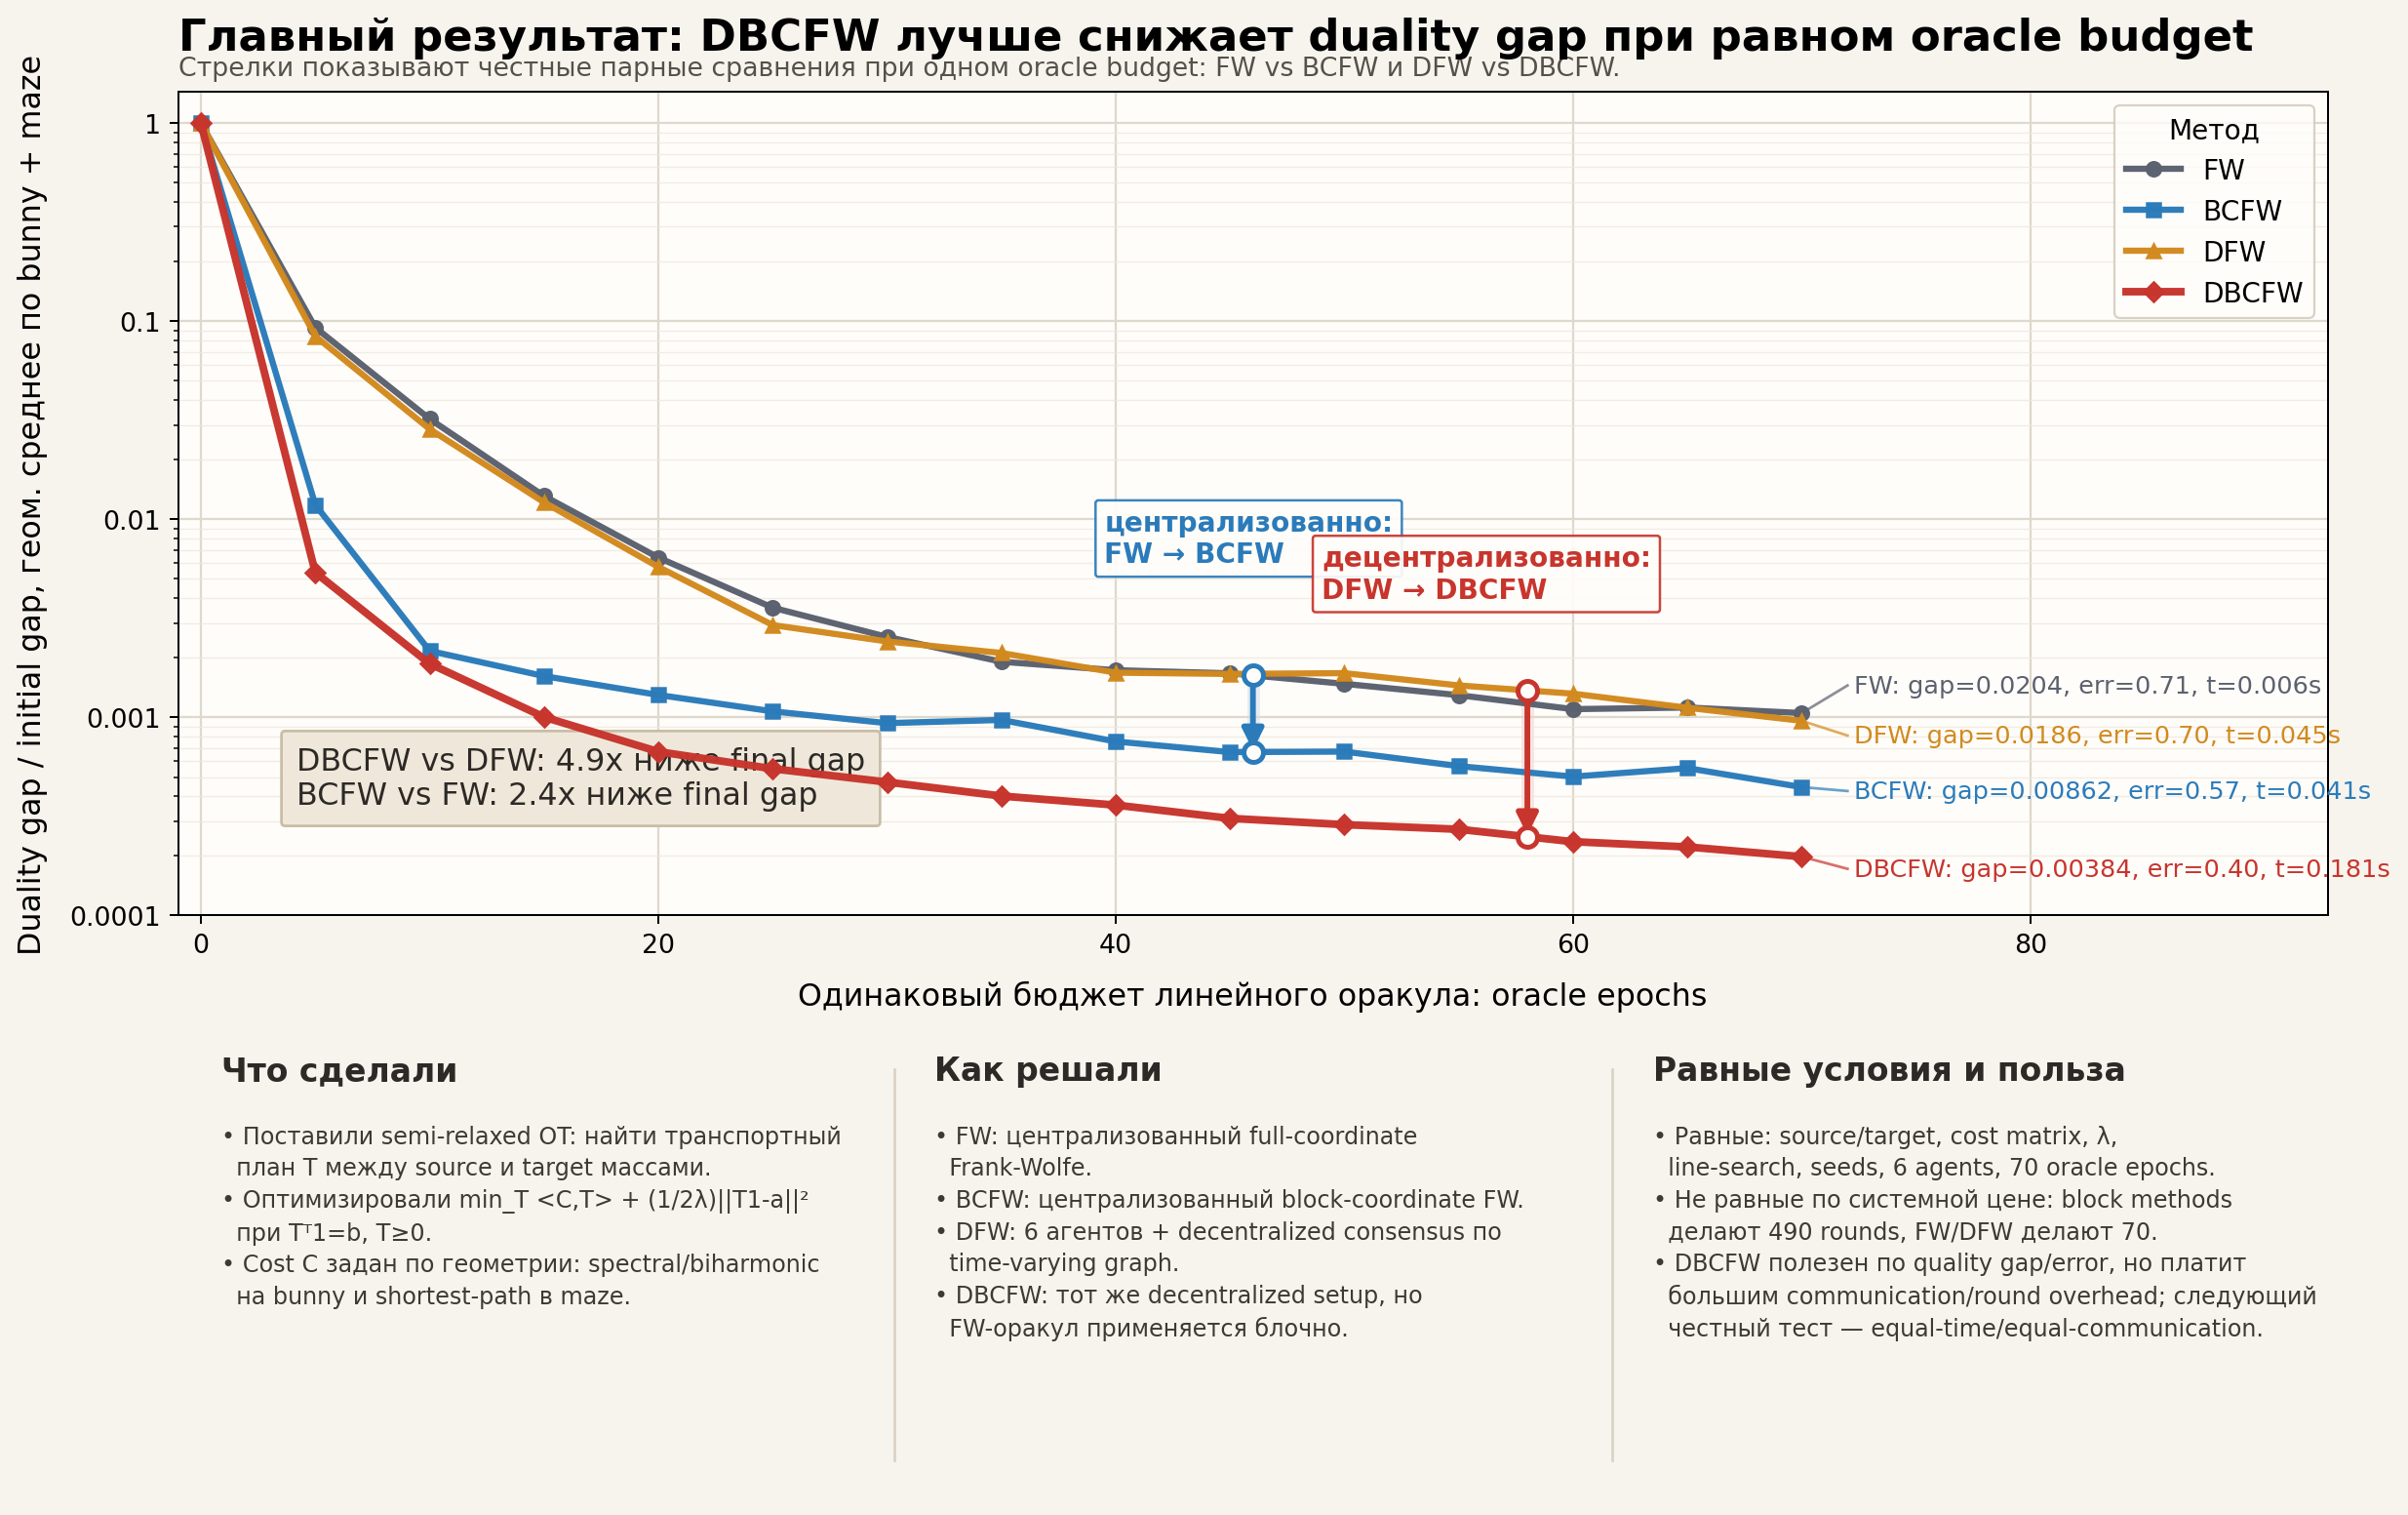
\includegraphics[width=\linewidth]{figures/main_result_one_graph_with_arrows.png}
  \caption{Главное сравнение на двух геометриях: 3D bunny и 2D maze. Метрика по оси \(y\) - normalized duality gap, усредненный геометрически по двум задачам. Синяя стрелка показывает эффект блочности в централизованном режиме (\method{FW}\(\to\)\method{BCFW}); красная - эффект блочности в decentralized режиме (\method{DFW}\(\to\)\method{DBCFW}).}
  \label{fig:main-result}
\end{figure}

\begin{table}[ht]
\centering
\small
\caption{Final metrics после 70 oracle epochs. Error - расстояние матрицы транспорта до reference optimum.}
\label{tab:final-metrics}
\begin{tabular}{llrrrrr}
\toprule
Setup & Method & Objective & Duality gap & Matrix error & Rounds & Time, s \\
\midrule
bunny & \method{FW}    & 0.296558 & 0.018686 & 0.666439 & 70  & 0.006 \\
bunny & \method{BCFW}  & 0.291102 & 0.009474 & 0.530041 & 490 & 0.045 \\
bunny & \method{DFW}   & 0.296859 & 0.017215 & 0.662091 & 70  & 0.047 \\
bunny & \method{DBCFW} & 0.289505 & 0.003920 & 0.358163 & 490 & 0.201 \\
\midrule
maze  & \method{FW}    & 0.353149 & 0.022255 & 0.750361 & 70  & 0.006 \\
maze  & \method{BCFW}  & 0.347231 & 0.007850 & 0.611315 & 420 & 0.036 \\
maze  & \method{DFW}   & 0.353971 & 0.020177 & 0.743209 & 70  & 0.042 \\
maze  & \method{DBCFW} & 0.344969 & 0.003763 & 0.448785 & 420 & 0.161 \\
\bottomrule
\end{tabular}
\end{table}

По геометрическому среднему final duality gap:
\[
  \frac{g_{\method{DFW}}}{g_{\method{DBCFW}}}\approx 4.85,
  \qquad
  \frac{g_{\method{FW}}}{g_{\method{BCFW}}}\approx 2.36.
\]
Средняя matrix error также уменьшается:
\[
  e_{\method{DFW}}\approx 0.70,\quad
  e_{\method{DBCFW}}\approx 0.40,
  \qquad
  e_{\method{FW}}\approx 0.71,\quad
  e_{\method{BCFW}}\approx 0.57.
\]
Таким образом, блочность полезна в обоих режимах, а в decentralized режиме дает наиболее сильный выигрыш по качеству решения.

\section{Как это связано с маршрутами на геометрии}

Решение \(T\) можно читать как дискретный flow plan:
\[
  \pi_T=\sum_{i=1}^{m}\sum_{j=1}^{n}T_{ij}\,\delta_{(x_i,y_j)}.
\]
Если \(T_{ij}>0\), часть массы идет из \(x_i\) в \(y_j\). Для визуализации строится маршрут \(\gamma_{ij}\) на геометрии и рисуется линия с толщиной/прозрачностью, пропорциональной \(T_{ij}\). На bunny маршруты идут по kNN-графу поверхности, на maze - по доступным клеткам лабиринта. Примеры reference routes показаны на рисунке \ref{fig:routes}.

\begin{figure}[ht]
  \centering
  \begin{minipage}{0.49\linewidth}
    \centering
    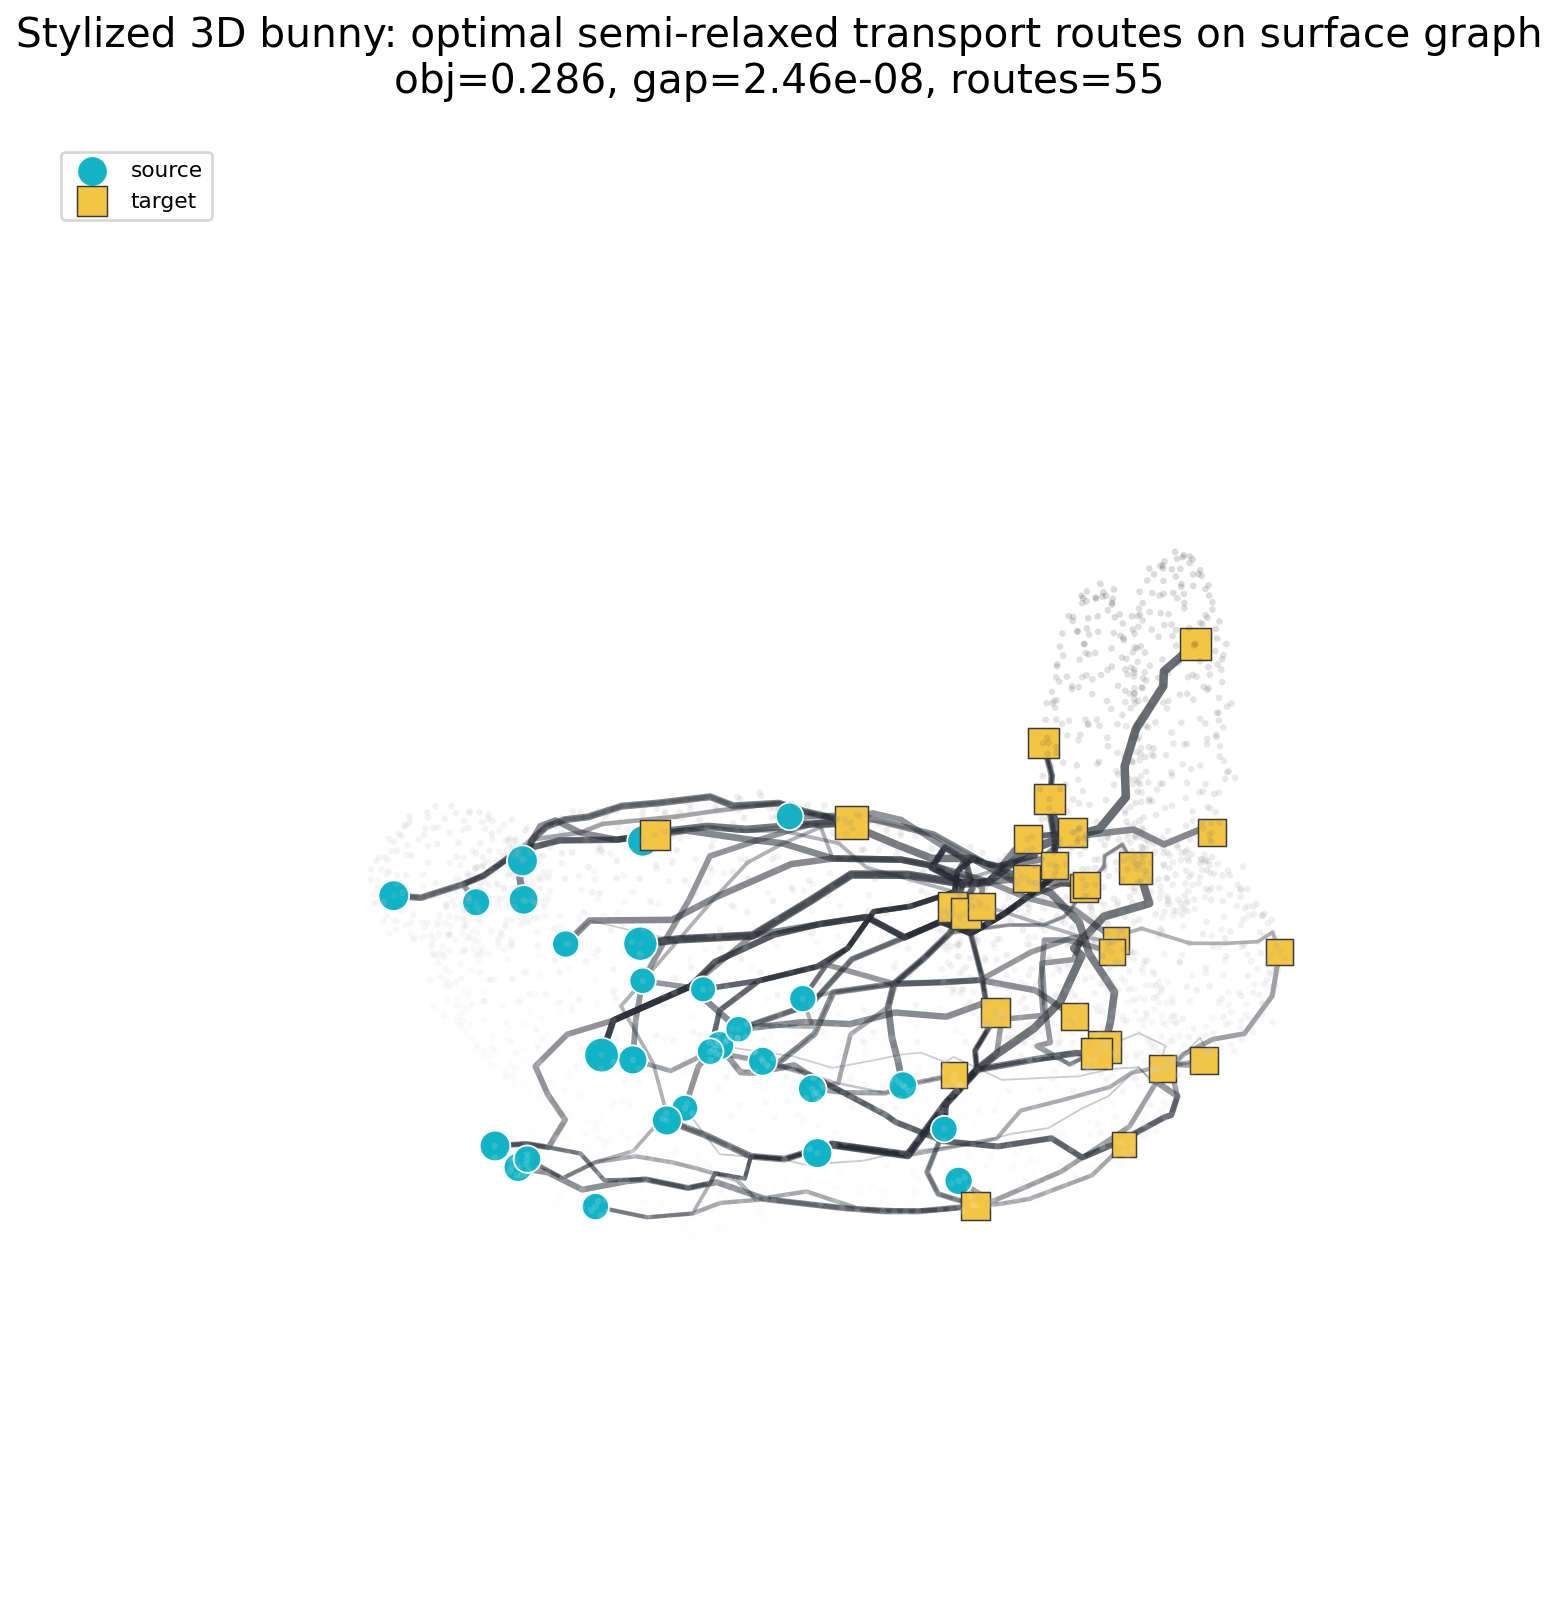
\includegraphics[width=\linewidth]{figures/bunny_3d_optimal_routes.png}
    \caption*{3D bunny: маршруты по поверхности}
  \end{minipage}
  \hfill
  \begin{minipage}{0.49\linewidth}
    \centering
    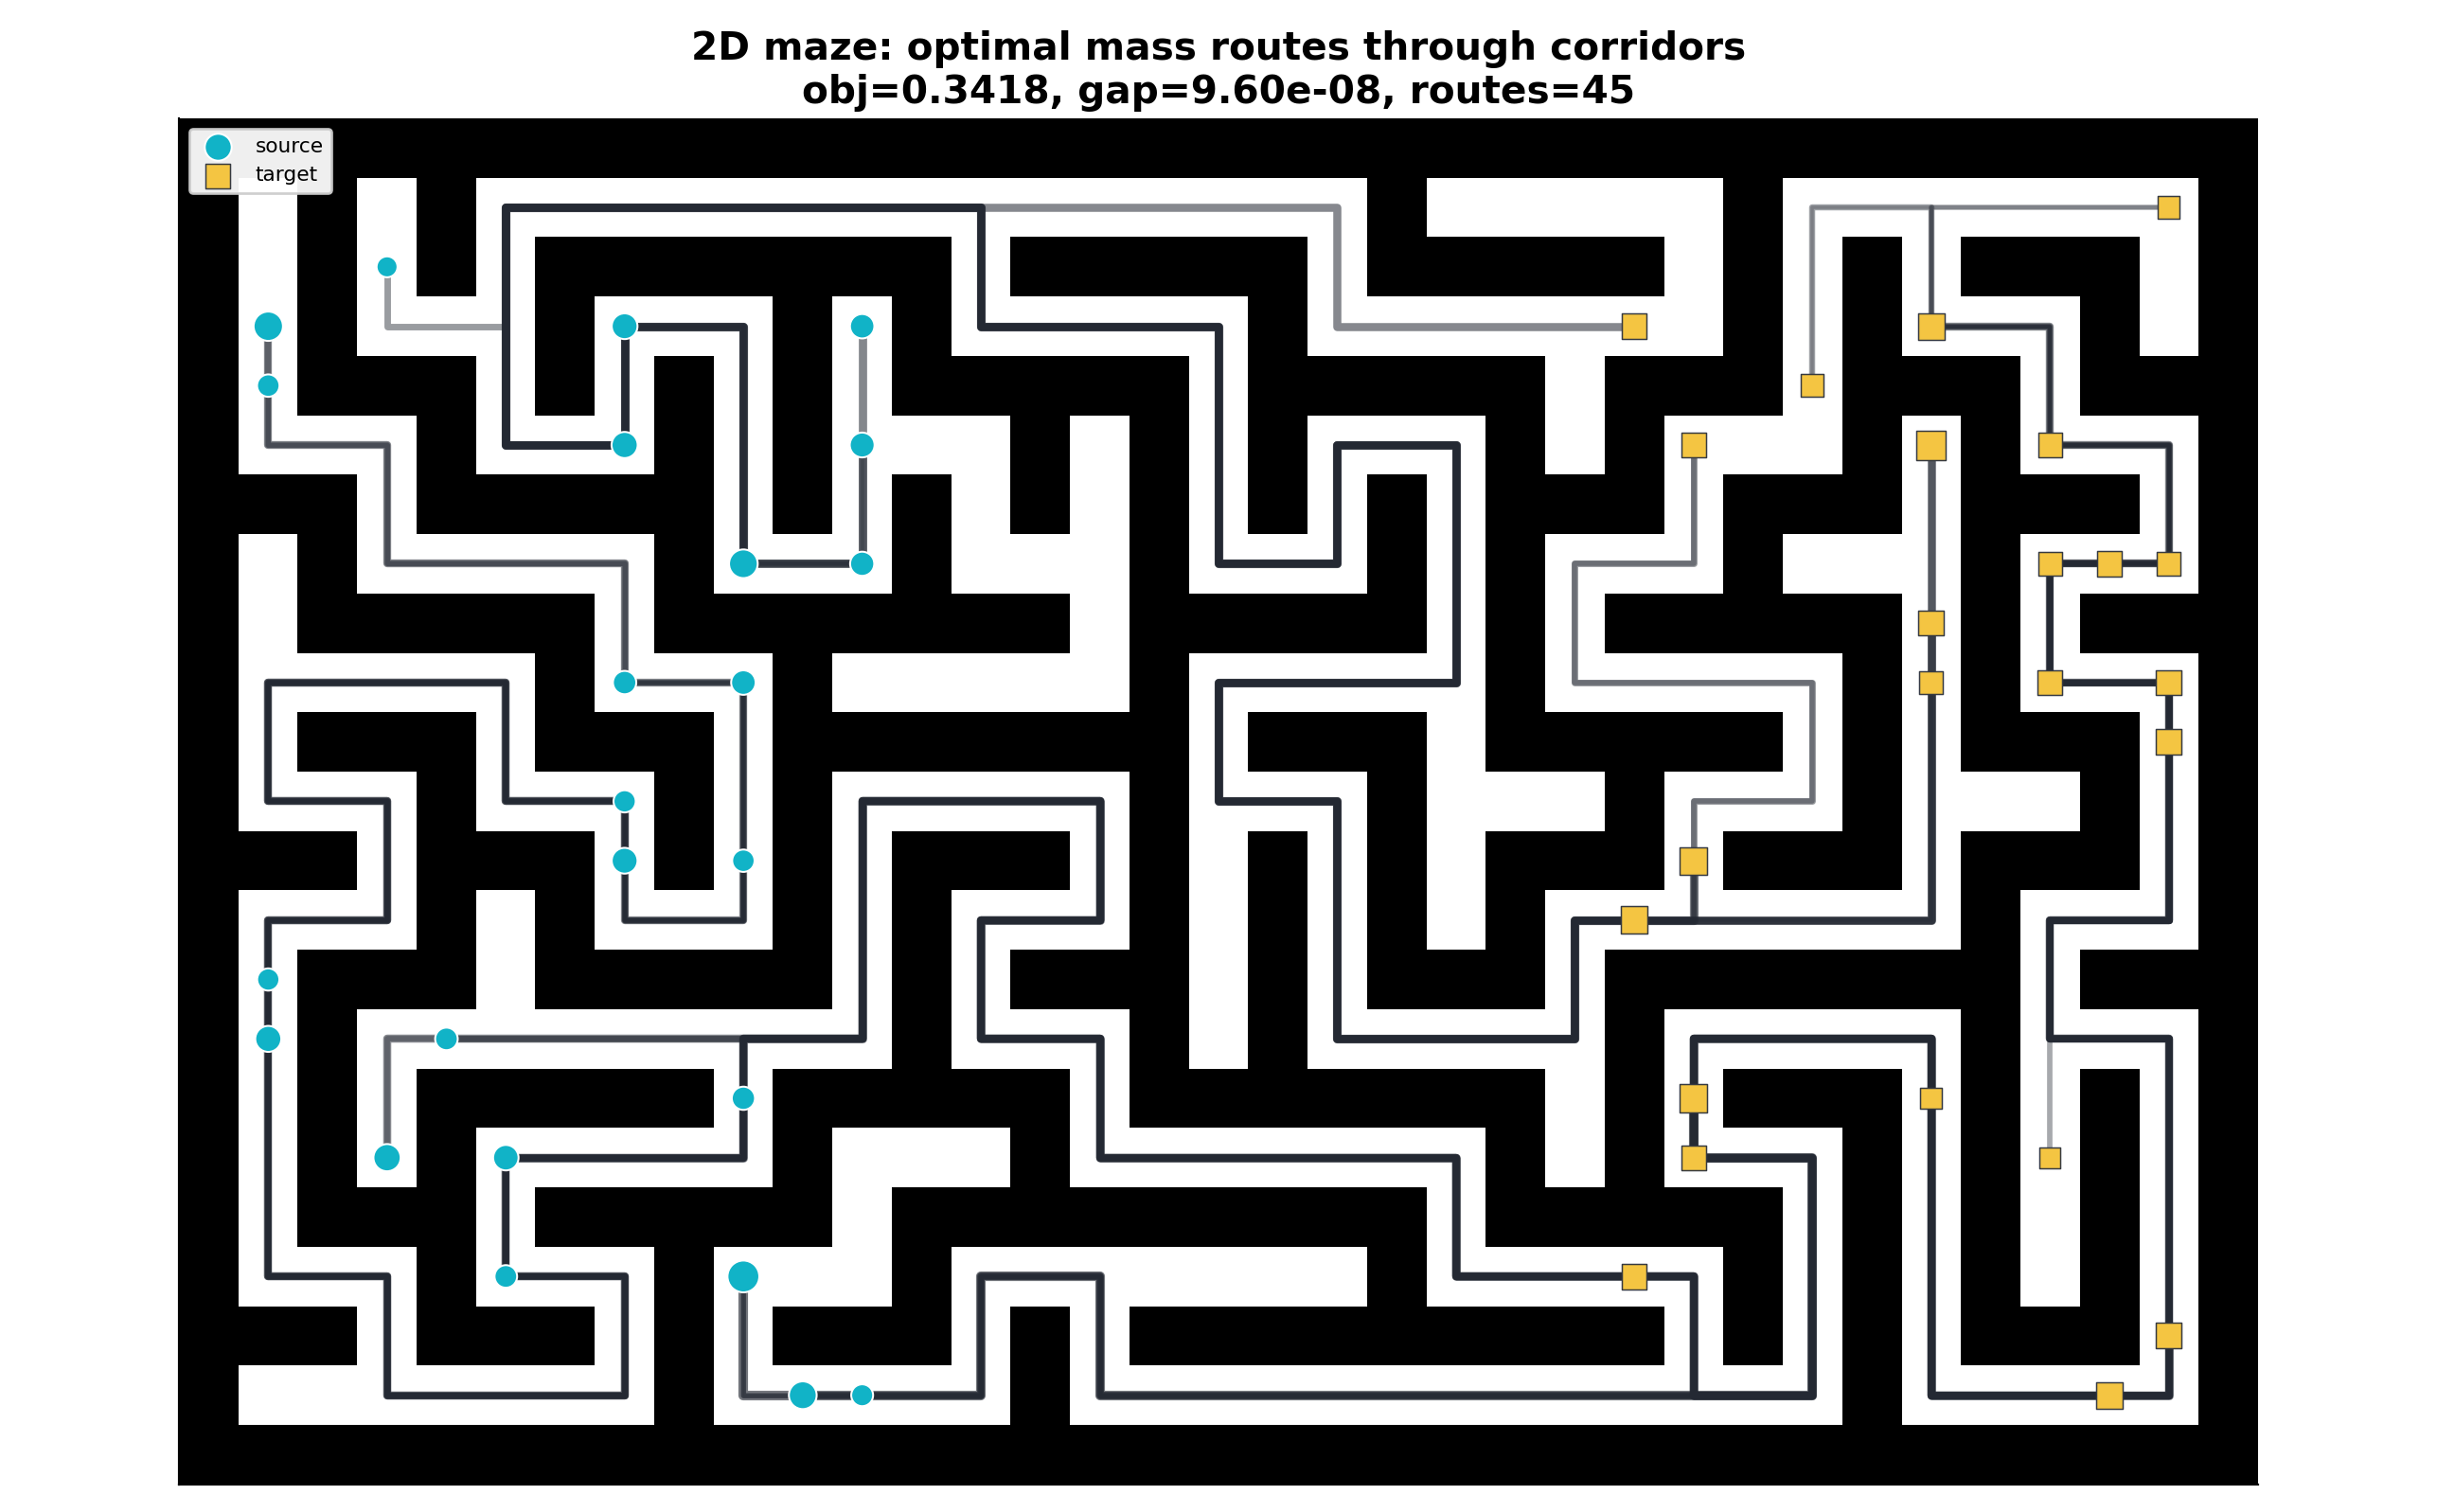
\includegraphics[width=\linewidth]{figures/maze_2d_optimal_routes.png}
    \caption*{2D maze: маршруты по коридорам}
  \end{minipage}
  \caption{Reference transport routes, используемые для интерпретации coupling как flow/matching планов.}
  \label{fig:routes}
\end{figure}

\section{Вывод}

В этом setup мы применили block-coordinate Frank-Wolfe к semi-relaxed OT subproblem, который возникает как дискретный matching/route planner для flow matching на общих геометриях. Сравнение показывает:
\begin{itemize}
  \item \method{BCFW} лучше \method{FW} по final gap при равном oracle budget;
  \item \method{DBCFW} лучше \method{DFW} по final gap и matrix error при равном oracle budget;
  \item эффект блочности особенно заметен в decentralized setup;
  \item цена улучшения - больше algorithm/communication rounds, поэтому next-step benchmark должен включать equal-time и equal-communication режимы.
\end{itemize}

Практическая интерпретация: \method{DBCFW} полезен, когда главная цель - получить более качественный sparse transport/matching plan при ограниченном oracle budget, а communication overhead допустим или может быть amortized. Если главный ресурс - wall-clock или communication rounds, текущих данных недостаточно для окончательной победы, и нужен отдельный budgeted benchmark.

\bibliographystyle{plainnat}
\bibliography{references}

\end{document}
